
\chapter{Paramagnetismo de Langevin} % Main chapter title

\begin{center}

Hay \\
Un magnetismo mental \\
Entre nosotros, \\
Que nos delata \\
A kilómetros de distancias. . . \\
Y usted lo sabe

\hspace{3.6cm} Marco Valerio\\

\end{center}


\section{Paramagnetismo de Langevin}

Es adecuado suponer a los átomos paramagnético como pequeños imanes, a veces, llamados agujas magnéticas, esta imagen es adecuado para describir el comportamiento de los átomos paramagnéticos a altas temperaturas, para lo cual debemos suponer que no existe ningún tipo de interacción entre ellos. Langevin fue el primero que formuló una teoría sobre el paramagnetismo. Trata a la sustancia como un conjunto clásico de dipolos magnéticos sin interacciones, con un tratamiento similar al problema de encontrar el momento dipolar eléctrico en un dieléctrico en presencia de un campo eléctrico. Sin campo magnético externo los dipolos están desordenados al azar; no existiendo un momento magnético neto. La introducción del campo magnético externo genera una inhomogeneidad en el espacio e introduce una fuerza ordenadora capaz de orientar los dipolos magnéticos. Como consecuencia aparece una magnetización resultante. Cuando desparece el campo externo la agitación térmica genera el estado inicial nuevamente, (ya que supusimos que no hay ningún tipo de interacción entre los dipolos magnéticos). Dicho de otro modo es una competencia entre la fuerza ordenadora, magnética y la acción desordenadora de la temperatura. De aquí inferimos que la magnetización depende de la temperatura. La idea es hallar el momento magnético resultante del material al introducir el campo.


\subsection{Energía del dipolo}

La energía de un dipolo magnético en un campo, cuyo vector inducción es $B$ está dada por, donde observamos que el valor mínimo de la energía se obtiene cuando $\theta=0$ razón por lo cual se orientan los dipolos.

\begin{equation}
	E_{\mu}=-\V{\mu}\cdot\V{B} -\lv{\mu}\lv{B}Cos(\theta) =-\mu_{0}\;\mu\;H\;Cos(\theta)
\end{equation}

Sumando las proyecciones, en la dirección del campo, de todos los momentos magnéticos de los átomos o moléculas obtendríamos el momento magnético total de la sustancia. Es razonable suponer que no todos los átomos reaccionaran de igual manera, luego estamos en presencia de un problema estadístico, con un gran numero de partículas (átomos). El momento magnético resultante será un equilibrio estadístico entre la acción orientadora del campo externo y la desorientadora debido al movimiento térmico El valor medio de las proyecciones de los momentos magnéticos individuales será la magnetización

\begin{equation}
	M=\left\langle \mu\;Cos(\theta) \right\rangle =\mu \left\langle Cos(\theta) \right\rangle
\end{equation}

Donde $N$ es el número de partículas por unidad de volumen, resta encontrar $\left\langle Cos(\theta) \right\rangle$ por ser un problema clásico podemos utilizar la distribución de Boltzmann que nos da la probabilidad de que el momento magnético este en un ángulo comprendido entre $\theta$ y $\theta + d\theta$ o lo que es equivalente dentro del ángulo sólido $\Omega$ como se observa en la figura. El ángulo sólido esta delimitado por la intercepción de dos conos sobre la esfera de radio $r$. El área de este sector es la longitud de la circunferencia cuyo radio es $2\pi r Sin(\theta)$ por la altura del sector $rd\theta$ o sea:

\begin{equation*}
	dS=2\pi r^{2}Sin(\theta)d\theta \quad \text{luego, tomando $r=1$ nos queda: } dS=2\pi Sin(\theta)d\theta = d\Omega
\end{equation*}

\begin{figure}[H]
    \centering
    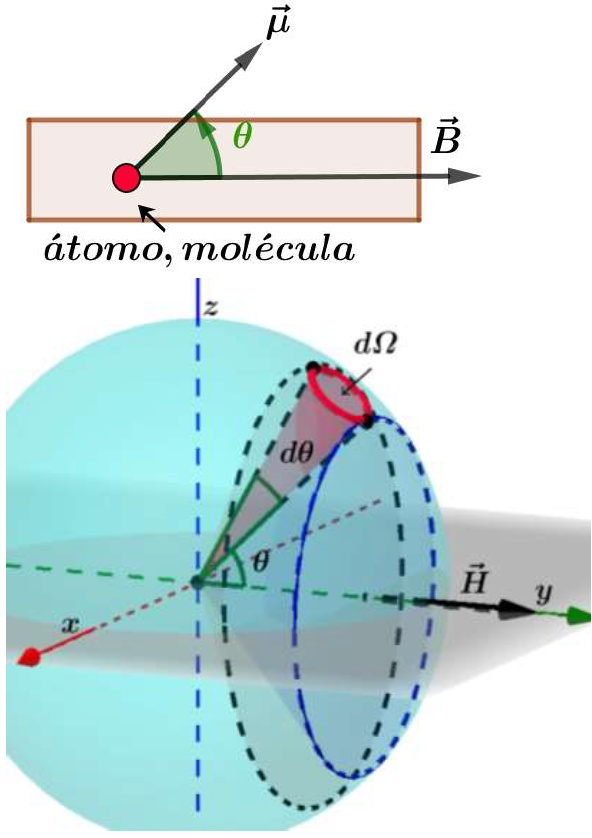
\includegraphics[width=0.6\textwidth]{./Figures/fig_c1}
	\caption{Momento magnético}
	\label{fig:c1}
\end{figure}

la probabilidad de una orientación para una dada energía es, 

\begin{equation}
	P(E)= \dfrac{\Bb{1}}{A'\;exp\left( \frac{E}{kT}\right) }
\end{equation}


donde $T$ es la temperatura en grados Kelvin, $k$ la constante de Boltzmann y $A'$ es una constante de normalización. No hay restricción sobre el número de partículas que pueden ocupar un dado estado Esta distribución es para partículas idénticas pero distinguibles. Luego:

\begin{equation}
	P(E)= A'\;exp\left( -\frac{E}{kT}\right) = A'\;exp\left( -\frac{\mu\mu_{0}\;N\;H\;Cos(\theta)}{kT}\right) = Ae^{\beta Cos(\theta)}
\end{equation}

Con $\Bb{\beta} =\left( -\frac{\mu\mu_{0}\;N\;H}{kT}\right)$ luego el valor medio será:

\begin{equation}
	M=\mu\langle Cos (\theta) \rangle= \mu \dfrac{\int Cos(\theta)exp(\beta Cos(\theta))d\Omega}{\int exp(\beta Cos(\theta))d\Omega}
\end{equation}

Extendida a todos los ángulos sólidos

\begin{equation}
\begin{aligned}
	M &= \mu \dfrac{\int_{0}^{2\pi} 2\pi Cos(\theta)exp(\beta Cos(\theta)) Sin(\theta)d\theta}{\int_{0}^{2\pi} 2\pi exp(\beta Cos(\theta)) Sin(\theta)d\theta}\\
	&= \mu \dfrac{\int_{0}^{2\pi} Cos(\theta)exp(\beta Cos(\theta)) d(Sin(\theta))}{\int_{0}^{2\pi} exp(\beta Cos(\theta)) d(Sin(\theta))}	\\
	&=
\mu \dfrac{\int_{-1}^{1} u\; exp(\beta u) du}{\int_{-1}^{1} exp(\beta u) du}	= \mu\dfrac{d}{d\beta}\left[ ln \left( \int_{-1}^{1} exp(\beta u) du \right)  \right] \\
	&= \mu \left[ \dfrac{e^{\beta}+e^{-\beta}}{e^{\beta}-e^{-\beta}}-\dfrac{1}{\beta} \right] \\
	&= \mu\left[ coth(\beta)-\dfrac{1}{\beta} \right] 
\end{aligned}
\end{equation}

La última expresión entre corchetes es llamada $L(\beta)$ función de Langevin.

Para valores pequeños de $\Bb{\beta} =\left( -\frac{\mu\mu_{0}\;N\;H}{kT}\right)$, o sea para $\mu\mu_{0}H < kT$ pequeños campos y temperaturas elevadas, podemos desarrollar la $Coth(\beta)= \dfrac{1}{\beta}+\dfrac{\beta}{3}+\dfrac{\beta^{3}}{45}+ \cdots$, luego si nos quedamos
con los dos primeros términos queda:

\begin{equation}
	M=\mu\langle Cos (\theta) \rangle= \mu \left[ Coth(\beta)-\dfrac{1}{\beta} \right] = \mu\dfrac{\beta}{3} = \dfrac{\mu^{2}\mu_{0}N}{3kT}
\end{equation}

luego la susceptibilidad paramagnética será

\begin{equation}
	\chi_{p} = \dfrac{M}{H} = \dfrac{\mu^{2}\mu_{0}N}{3kT}
\end{equation}

Esta expresión concuerda con la ley experimental llamada de Curie que nos indica que $\chi_{p}=\dfrac{c}{T}$

\begin{equation*}
\text{Langevin aplica} \rightarrow
				\begin{cases}
  				\text{Bien en: vapores y gases paramagneticos} \\
 				\text{Bien en: sales y metales a altas temperaturas} \\
  				\text{Mal en: metales paramagnetico sólidos}
    			\end{cases}
\end{equation*}

Es razonable pensar que los resultados en los sólidos metálicos no sean adecuados, puesto que unas de las premisas supuestas es que no existía interacción entre las partículas, cosa que evidentemente no es así. La suposición de un gas sin interacción entre partículas deja de ser valida. Pero, si la temperatura es elevada, la energía de las partículas supera a la de interacción entre ellas y modelo de gas es valido.

En la figura \ref{fig:c2} se observa representada la función de Langevin y la recta que se le aproxima para pequeños valores de $\beta$ La zona rayada indica su límite. Las deducciones anteriores se realizaron para la región donde rige la aproximación $\mu\mu_{0}H < kT$. Si contrariamente nos ubicamos donde vale $\mu\mu_{0}H >> kT$ entonces, $\beta\rightarrow\infty$ o sea, un valor muy grande, entonces, la ecuación

\begin{equation*}
	M= \mu \left[ Coth(\beta)-\dfrac{1}{\beta} \right] \approx \mu
\end{equation*}

Por tanto a temperaturas muy bajas la susceptibilidad paramagnética disminuye a medida que aumenta el campo. 

\begin{equation}
	\chi_{p} = \dfrac{M}{H} \approx \dfrac{\mu}{H}\rightarrow 0
\end{equation}


Con el objeto de contemplar la interacción atómica existente en los solidos metálicos, Weiss introdujo la idea de que a consecuencia de la interacción entre los momentos magnéticos se genera un muevo campo interno O sea los átomos individuales interactuaban entre sí a través de un campo interno Weiss lo llamó "campo molecular“ y lo supuso igual a: $\alpha M$.


\begin{figure}[H]
    \centering
    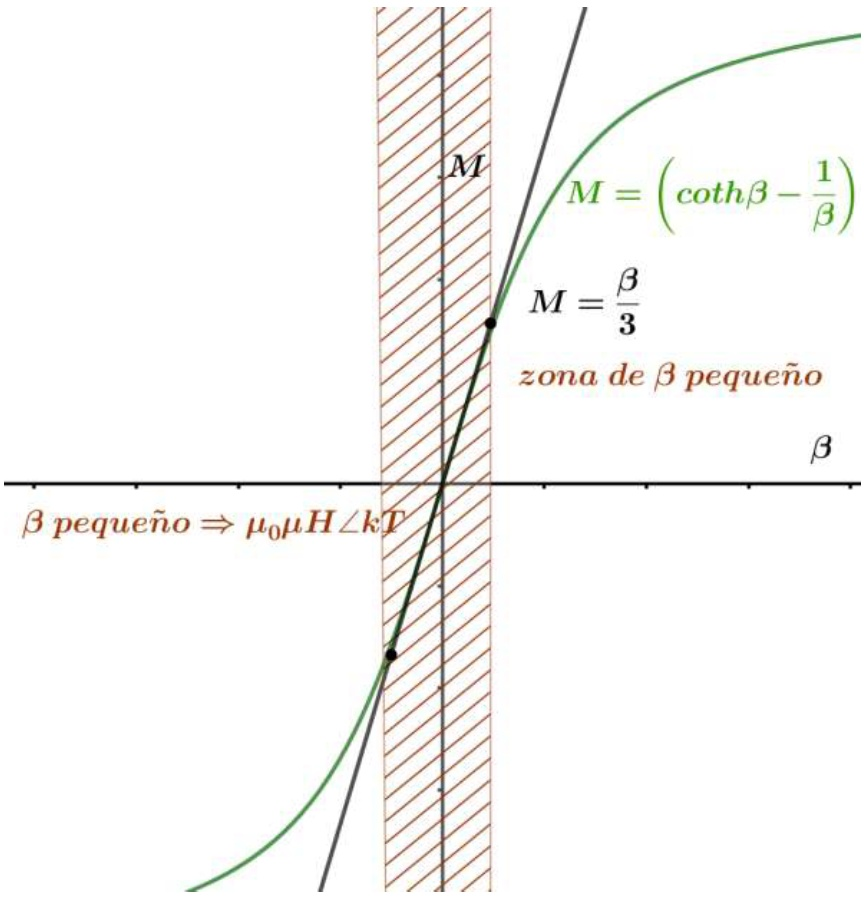
\includegraphics[width=0.6\textwidth]{./Figures/fig_c2}
	\caption{Función de Langevin}
	\label{fig:c2}
\end{figure}

Luego, si al campo externo $H$ le sumamos el interno, nos da el efectivo o total $H_{ef}=H+\alpha H$ si esta expresión la reemplazamos en:

\begin{equation}
\begin{aligned}
M &= \dfrac{\mu^{2}\mu_{0}N}{3kT}H =\dfrac{\mu^{2}\mu_{0}N}{3kT}(H+\alpha M) \\
  &= \dfrac{\mu^{2}\mu_{0}N}{3kT}H+ \alpha\dfrac{\mu^{2}\mu_{0}N}{3kT}M
  = M\left(1-\alpha\dfrac{\mu^{2}\mu_{0}N}{3kT} \right)
\end{aligned}
\end{equation}

Por lo que resulta que:

\begin{equation}
  \chi_{p}=\dfrac{M}{H}= \dfrac{\dfrac{\mu^{2}\mu_{0}N}{3kT}}{\left(1-\alpha\dfrac{\mu^{2}\mu_{0}N}{3kT} \right)}=\dfrac{\mu^{2}\mu_{0}N}{3k \left(T-\alpha\dfrac{\mu^{2}\mu_{0}N}{3k} \right)}= \dfrac{\alpha}{T-\theta}
\end{equation} 

Que es la ley de Curie Weiss donde $\alpha=\dfrac{\mu^{2}\mu N}{3k}$ y $\theta=\alpha^{2}$ llamada temperatura de Curie $T_{c}$ y marca el límite entre el estado paramagnético y ferromagnéticos del material. Este desarrollo muestra que un sólido paramagnético con momentos atómicos  localizados pero interactivos tendrá una susceptibilidad que obedece a la ley de Curie-Weiss.

\begin{figure}[H]
    \centering
    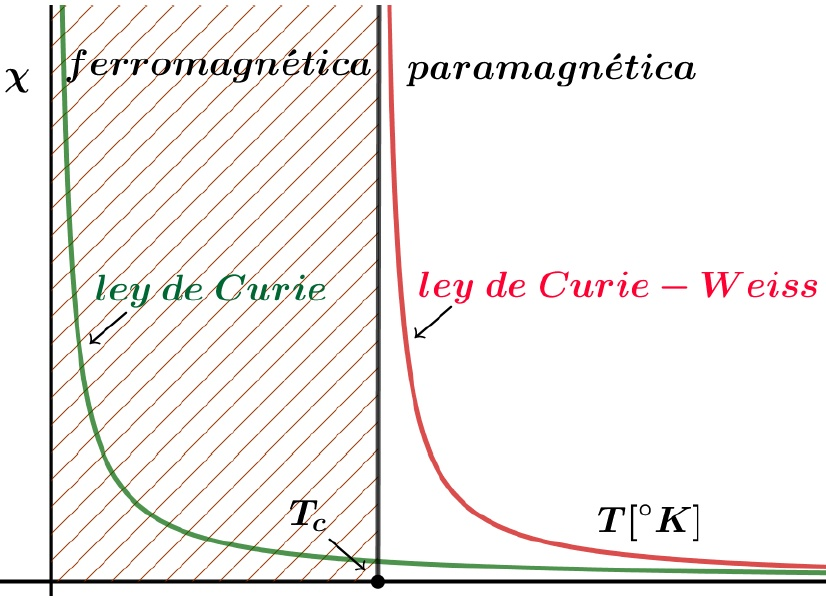
\includegraphics[width=0.6\textwidth]{./Figures/fig_c3}
	\caption{Ley de Curie-Wiess}
	\label{fig:c3}
\end{figure}
